\icode{E-MV-MU-L3-260625-002}
（多选）
如图所示，倾角为\(\theta =\)\,\qty{30}{\degree}的足够长光滑绝缘斜面固定在水平面上，空间中存在水平向右的匀强电场，电场强度\(E = \frac{\sqrt{3}mg}{3q} \)。小球\(A\)的电荷量为\( + q\)(\(q > 0\))，小球\(B\)不带电，质量均为\(m\)，两球用劲度系数为\(k\)的轻质绝缘弹簧连接，弹簧处于原长并锁定。现解除锁定释放两球并开始计时，\(t_0\)时刻两球第一次速度相等，速度大小为\(v_0\)，此时弹簧形变量为\(x_0\)，在整个运动过程中弹簧均在弹性限度内，重力加速度为\(g\)。下列说法正确的是\paren[]

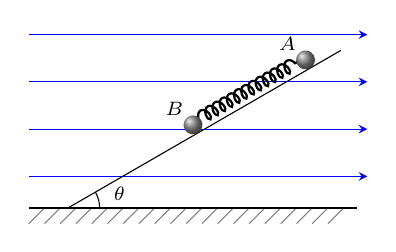
\begin{tikzpicture}[font=\scriptsize]
    \foreach \y in{.4,1,...,2.5}
        \draw[-stealth,blue] (-.5,\y)--(3.8,\y);
	\def\TheTa{30}%旋转角度
	\def\LenGth{4}%斜面长度
	\pgfmathsetmacro\CosLenGth{\LenGth*cos(\TheTa)}
	\begin{scope}[rotate=\TheTa]	
		\draw (0,0)--++(\LenGth,0);
        \draw[thick,decoration={aspect=.6,segment length=3,amplitude=.8mm,coil},decorate] (2,.15)--(3.5,.15);
        \shade[ball color=gray] (1.9,.12)node[above left,black]{\(B\)} circle(.12);
        \shade[ball color=gray] (3.55,.12)node[above left,black]{\(A\)} circle(.12);
	\end{scope}
	\draw (.4,0) arc(0:\TheTa:.4);
	\node at(.65,.18){\(\theta\)};
	\foreach \x in{-.5,-.3,...,\CosLenGth}
		\draw[gray] (\x,-.2)--++(.2,.2);
	\draw[thick] (-.5,0)--({\CosLenGth+.2},0);
\end{tikzpicture}
\begin{choices}
    \item 两球每次加速度相同时弹簧的形变量均为\(\frac{mg}{4k}\)
    \item 两球每次速度相同弹簧形变量均为\(x_0\)
    \item 在\(t = t_0\)时，小球\(A\)的电势能增加了\(\frac{mg}{8}(v_0t_0 - x_0)\)
    \item 在\(t = 2t_0\)时，两球和弹簧系统机械能减少了\(mgv_0t_0\)
\end{choices}
\begin{answer}
    AD\quad 提示：两球质心做匀加速运动，\(a_c = \frac{\frac{1}{2}mg}{2m} = \frac{1}{4}g\)
\end{answer}